%% abtex2-modelo-relatorio-tecnico.tex, v-1.9.6 laurocesar
%% Copyright 2012-2016 by abnTeX2 group at http://www.abntex.net.br/ 
%%
%% This work may be distributed and/or modified under the
%% conditions of the LaTeX Project Public License, either version 1.3
%% of this license or (at your option) any later version.
%% The latest version of this license is in
%%   http://www.latex-project.org/lppl.txt
%% and version 1.3 or later is part of all distributions of LaTeX
%% version 2005/12/01 or later.
%%
%% This work has the LPPL maintenance status `maintained'.
%% 
%% The Current Maintainer of this work is the abnTeX2 team, led
%% by Lauro César Araujo. Further information are available on 
%% http://www.abntex.net.br/
%%
%% This work consists of the files abntex2-modelo-relatorio-tecnico.tex,
%% abntex2-modelo-include-comandos and abntex2-modelo-references.bib
%%

% ------------------------------------------------------------------------
% ------------------------------------------------------------------------
% abnTeX2: Modelo de Relatório Técnico/Acadêmico em conformidade com 
% ABNT NBR 10719:2015 Informação e documentação - Relatório técnico e/ou
% científico - Apresentação
% ------------------------------------------------------------------------ 
% ------------------------------------------------------------------------

\documentclass[
	% -- opções da classe memoir --
	12pt,				% tamanho da fonte
	article,			% não quebra páginas em novos capitulos
	openright,			% capítulos começam em pág ímpar (insere página vazia caso preciso)
	%twoside,			% para impressão em recto e verso. Oposto a oneside
	oneside,
	a4paper,			% tamanho do papel. 
	% -- opções da classe abntex2 --
	chapter=TITLE,		% títulos de capítulos convertidos em letras maiúsculas
	section=TITLE,		% títulos de seções convertidos em letras maiúsculas
	%subsection=TITLE,	% títulos de subseções convertidos em letras maiúsculas
	%subsubsection=TITLE,% títulos de subsubseções convertidos em letras maiúsculas
	% -- opções do pacote babel --
	english,			% idioma adicional para hifenização
	french,				% idioma adicional para hifenização
	spanish,			% idioma adicional para hifenização
	brazil,				% o último idioma é o principal do documento
]{abntex2}


% ---
% PACOTES
% ---

% ---
% Pacotes fundamentais 
% ---
\usepackage{lmodern}			% Usa a fonte Latin Modern
\usepackage[T1]{fontenc}		% Selecao de codigos de fonte.
\usepackage[utf8]{inputenc}		% Codificacao do documento (conversão automática dos acentos)
\usepackage{indentfirst}		% Indenta o primeiro parágrafo de cada seção.
\usepackage{color}				% Controle das cores
\usepackage{graphicx}			% Inclusão de gráficos
\usepackage{microtype} 			% para melhorias de justificação
% ---

% ---
% Pacotes adicionais, usados no anexo do modelo de folha de identificação
% ---
\usepackage{multicol}
\usepackage{multirow}
% ---

% ---
% Pacotes adicionais
% ---
\usepackage{placeins}	% permite usar 
\usepackage{wrapfig} % Permite textos em volta de figuras
\usepackage{pdfpages} % Permite usar o \includepdf
% ---

% ---
% Pacotes de citações
% ---
\usepackage[brazilian,hyperpageref]{backref}	 % Paginas com as citações na bibl
\usepackage[alf]{abntex2cite}	% Citações padrão ABNT

% ---
% Pacotes de códigos fonte
% ---
\usepackage{listingsutf8}

% Pacote para desenho de blocos
\usepackage{schemabloc}
\usetikzlibrary{circuits}

% --- 
% CONFIGURAÇÕES DE PACOTES
% --- 

% ---
% Configurações do pacote backref
% Usado sem a opção hyperpageref de backref
\renewcommand{\backrefpagesname}{Citado na(s) página(s):~}
% Texto padrão antes do número das páginas
\renewcommand{\backref}{}
% Define os textos da citação
\renewcommand*{\backrefalt}[4]{
%	\ifcase #1 %
%	Nenhuma citação no texto.%
%	\or
%	Citado na página #2.%
%	\else
%	Citado #1 vezes nas páginas #2.%
%	\fi
}%
% ---

% ---
% Informações de dados para CAPA e FOLHA DE ROSTO
% ---
\titulo{PROJETO E IMPLEMENTAÇÃO DE CONTROLADOR DIGITAL UTILIZANDO ALOCAÇÃO DE POLOS}
\autor{João Antônio Cardoso}
\local{Florianópolis}
\data{\today}
%\data{2015, v-1.9.6}
\orientador[Prof. ]{Flábio Alberto Bardemaker Batista}
\instituicao{Instituto Federal de Educação, Ciência e Tecnologia de Santa Catarina - Campus Florianópolis \\
	Engenharia Eletrônica \\
	Sistemas de Controle II
}
\tipotrabalho{Relatório técnico}
% O preambulo deve conter o tipo do trabalho, o objetivo, 
% o nome da instituição e a área de concentração 
\preambulo{\@title - relatório técnico para aprovação na parte laboratorial da disciplina de Sistemas de Controle II.}
% ---

% ---
% Configurações de aparência do PDF final

% alterando o aspecto da cor azul
\definecolor{blue}{RGB}{41,5,195}

% informações do PDF
\makeatletter
\hypersetup{
	pdftitle={\@title},
	pdfauthor={\@author},
	pdfsubject={\imprimirpreambulo},
	pdfcreator={LaTeX},
	colorlinks=true,       		% false: boxed links; true: colored links
	linkcolor=blue,          	% color of internal links
	citecolor=blue,        		% color of links to bibliography
	filecolor=magenta,      	% color of file links
	urlcolor=blue
}
\makeatother
% --- 

% ---
% Modificando a capa padrão
% ---
\renewcommand{\imprimircapa}{
	\begin{capa}
		\SingleSpacing
		\begin{adjustwidth}{}{}			
			\begin{minipage}{1\textwidth}
				\begin{wrapfigure}{l}{0.25\textwidth}
					\vspace*{-1em}\includegraphics[height=4em]{logotipo_ifsc.jpg}
				\end{wrapfigure}
				\imprimirinstituicao 
			\end{minipage}
			\vfill
			\begin{center}\ABNTEXchapterfont\LARGE\imprimirtitulo
				\vfill
				\small
				\begin{center}
					Aluno: \imprimirautor\\[1em]
					\imprimirorientadorRotulo\imprimirorientador\\
					\imprimircoorientadorRotulo\imprimircoorientador
				\end{center}
				\vfill
				\imprimirlocal, \imprimirdata
			\end{center}	
		\end{adjustwidth}
	\end{capa}
}

% --- 
% Espaçamentos entre linhas e parágrafos 
% --- 

% O tamanho do parágrafo é dado por:
\setlength{\parindent}{1.3cm}

% Controle do espaçamento entre um parágrafo e outro:
\setlength{\parskip}{0.2cm}  % tente também \onelineskip

% ---
% compila o indice
% ---
\makeindex
% ---

% ----
% Início do documento
% ----
\begin{document}
	
	% Seleciona o idioma do documento (conforme pacotes do babel)
	%\selectlanguage{english}
	\selectlanguage{brazil}
	
	% Retira espaço extra obsoleto entre as frases.
	\frenchspacing 
	
	% ----------------------------------------------------------
	% ELEMENTOS PRÉ-TEXTUAIS
	% ----------------------------------------------------------
	% \pretextual
	
	% ---
	% Capa
	% ---
	\imprimircapa
	% ---
	
	% ---
	% inserir o sumario
	% ---
	\pdfbookmark[0]{\contentsname}{toc}
	\tableofcontents*
	%\cleardoublepage
	% ---
	
	% ---
	% inserir lista de figuras
	% ---
	\clearpage
	\listoffigures
	\vspace{34pt}
	\listoftables
	
	% ----------------------------------------------------------
	% ELEMENTOS TEXTUAIS
	% ----------------------------------------------------------
	\textual
	
	\pagebreak
	
	% ----------------------------------------------------------
	% Introdução (exemplo de capítulo sem numeração, mas presente no Sumário)
	% ----------------------------------------------------------
	\chapter*[Introdução]{Introdução}
	\addcontentsline{toc}{chapter}{Introdução}
	
    Este trabalho apresenta um relatório do processo de solução do primeiro trabalho da disciplina de Sistemas de Controle II, no qual se pretende projetar e implementar um controlador digital, da teoria à prática laboratorial.
	
	\section[Objetivos]{Objetivos}
	
	A partir de um enunciado explicando a proposta de trabalho disponibilizada pelo professor, o autor propõe os seguintes itens como objetivos deste trabalho:
	
	\begin{itemize}
	    \item Fabricar uma planta para ser controlada.
	    \item Identificar a função de transferência equivalente da planta.
	    \item Especificar os requisitos do projeto.
	    \item Projetar um controlador utilizando alocação de polos.
	    \item Implementar o controlador em um \textit{microcontrolador}.
	    \item Avaliar o funcionamento da solução implementada.
		\item (opção do autor) Desenvolver o projeto utilizando somente softwares gratuitos, respeitando suas licenças de uso, dando preferência para softwares de código aberto.
	\end{itemize}
	
	\section[Desenvolvimento]{Desenvolvimento}

    	Como objeto de estudo, uma planta para ser controlada foi proposta pelo professor, e modificada de acordo com a disponibilidade de componentes e também modificada para a utilização de alimentação simples ao invés de alimentação simétrica, facilitando a montagem, que desta forma pode ocorrer diretamente por uma porta USB 1.0, comum em nossas ferramentas de trabalho como osciloscópios e computadores.
    	
    	Por se tratar de um projeto de controle digital, o autor optou por utilizar um \textit{DSP} \textit{TMS320F28335} da \textit{Texas Instruments} como controlador, imbutido em um \textit{Control Card}, conectado à um kit de desenvolvimento chamado \textit{C2000 Peripheral Explorer Kit}.
    	
    	\subsection{Descrição da Planta}
    	
        	A planta resultante (\autoref{fig-planta}) consiste em três nós que são interconectados por meio de dois blocos. O bloco entre os nós \textbf{A} e \textbf{B} pode ser compreendido como um filtro passa-baixa de primeira ordem ativo de ganho unitário. O segundo bloco, entre os nós \textbf{B} e \textbf{C}, pode ser compreendido como um filtro passa-baixa de segunda ordem ativo de ganho unitário, utilizando uma topologia conhecida como \textit{Sallen-key}. 
        	
        	\begin{figure}[htbp]
        		\centering
        		\caption{Planta}
        		\includegraphics[width=\textwidth,height=240px,keepaspectratio]{imgs/planta.png}
        		\label{fig-planta}
        		\legend{Fonte: do autor. }
        	\end{figure}
        	
        	Como o amplificador operacional do primeiro bloco fornece a característica de alta impedância na entrada e baixa impedância na saída, podemos caracterizar os dois blocos separadamente. Sendo assim, as funções de transferência dos blocos, e também da planta completa (do nó \textbf{A} à \textbf{C}), podem ser descritas como nas Equações \ref{eq-tfb1}, \ref{eq-tfb2} e \ref{eq-tfplanta}, respectivamente.
        	
        	\begin{eqnarray}
        		\label{eq-tfb1}
        		H_{AB} = \frac{V_B}{V_A} = \frac{\frac{1}{R_3C_3}}{s+\frac{1}{R_3C_3}} \\
        		\label{eq-tfb2}
        		H_{BC} = \frac{V_C}{V_B} = \frac{\frac{1}{R_1C_1R_2C_2}}{s^2 +s\,(\frac{1}{R_1C_1}+\frac{1}{R_2C_2}) + \frac{1}{R_1C_1R_2C_2}} \\
        		\label{eq-tfplanta}
        		H_{AC} = \frac{V_C}{V_A} = H_{AB}\,H_{BC} = \frac{\frac{1}{R_3C_3}}{s+\frac{1}{R_3C_3}}\,\frac{\frac{1}{R_1C_1R_2C_2}}{s^2 +s\,(\frac{1}{R_1C_1}+\frac{1}{R_2C_2}) + \frac{1}{R_1C_1R_2C_2}}
        	\end{eqnarray}
        	
        	Considerando resistores de 10\% e capacitores de 20\% de tolerância, foi realizada uma análise combinacional dos valores máximos, mínimos e nominais, por meio de um \textit{script} em \textit{Python} para que se compreendesse o conjunto possíveis de respostas do sistema, nesta análise inicial foi gerado um gráfico (\ref{fig-step-tolerancias}).
        	
        	\begin{figure}[htbp]
        		\centering
        		\caption{Resposta ao degrau considerando tolerâncias}
        		\includegraphics[width=\textwidth,height=240px,keepaspectratio]{tex/imgs/ftma/step-tolerancias.png}
        		\label{fig-step-tolerancias}
        		\legend{Fonte: do autor. }
        	\end{figure}
        	
        	A partir do esquemático da planta (\autoref{fig-planta}), um novo esquemático foi desenhado no software de projeto de placas de circuito impresso \textit{KiCAD}, contendo pontos de teste, conectores e \textit{jumpers} para facilitar o teste dos blocos isoladamente. Para tal esquemático, \textit{layout} foi desenhado, e a placa manufaturada.
        	
            Como projetar um controlador que funcione para toda a gama de tolerância dos componentes está fora do contexto desta disciplina, vamos projetar um controlador especificamente para este exemplar manufaturado. Para tal, é necessário levantar sua função de transferência equivalente.
    	
    	\subsection{Identificação da Planta}
    	
        	Uma técnica para a identificação da planta pode ser aplicar um sinal conhecido e a partir de figuras de mérito, levantar seus parâmetros e equacionar uma função de transferência de segundo grau equivalente.
        	
        	Por se tratar de uma planta que trabalha em uma região de tensão positiva na entrada e saída, e também por sabermos que o circuito possui não linearidades próximo aos valores de sua alimentação, aqui iremos aplicar um degrau de 1 à $1.5\,[V]$, ou seja, não é um degrau unitário, mas é um sinal conhecido e tomando alguns cuidados, toda a teoria que utiliza degraus unitários pode ser utilizada.
        	
        	Para deixar explícito como foram computadas as figuras de mérito, as Equações \ref{eq-mp} à \ref{eq-settling_time} descrevem o modo com que foram calculados os valores de \textit{Tempo de Subida} (\textit{Rise Time} - $t_r$) \textit{Sobressinal} (\textit{Overshoot} - $Mp$), o \textit{Tempo de Acomodação em 5\%} (Settling Time - $t_{s_{5\%}}$ ).
        	
        	\begin{eqnarray}
        		\nonumber
        		V_{10\%} = 0,1\cdot(\;V_{\infty} -V_{0}\;) \\
        		\nonumber
        		V_{90\%} = 0,9\cdot(\;V_{\infty} -V_{0}\;) \\
        		\label{eq-mp}
        		t_{r} = t_{(V_{90\%})} - t_{(V_{10\%})} \\
        		\nonumber
        		V_{max_{5\%}} \leq (1 +0.05) \cdot (V_{(\infty)} - V_{0}) +V_{0} \\
        		\nonumber
        		V_{min_{5\%}} \leq (1 -0,05) \cdot (V_{(\infty)} - V_{0}) +V_{0} \\
        		\label{eq-settling_time}
        		t_{s_{5\%}} = max\left(\; t_{(Vmax_{5\%})}\quad, \quad t_{(Vmin_{5\%})}\;\right)		
        	\end{eqnarray}
        	
        	Antes de realizar as medições, a primeira etapa foi executar a auto-calibração do osciloscópio e calibrar manualmente as ponteiras, para garantir que não houvessem erros técnicos nas medições.
        	
        	Com o osciloscópio devidamente calibrado, verificou-se o sinal \textit{PWM} de entrada, se estava na frequência de operação correta, e se estava nos ciclos-tarefa como foi calculado. 
        	
        	O gatilho do osciloscópio foi configurado no canal 2, que mostra o momento em que o degrau é aplicado, portanto, todas as medidas de tempo com os cursores são relativos ao tempo em que o degrau foi aplicado, que será considerado como o tempo inicial ($t_0=0\,[s]$).
        	
        	A primeira ponteira do osciloscópio foi então conectada na saída da planta. O resultado é mostrado na \autoref{fig-ftma-step}.
        	
        	Para medir com maior precisão, optou-se por trabalhar com o diferentes escalas do osciloscópio para focar em cada parte da forma de onda. A fim de alcançar uma precisão ainda melhor no osciloscópio, foi utilizado o \textit{trigger} no \textit{modo normal}, que permitiu que a função de média de 128 amostras na aquisição atuasse como uma sobre-amostragem, adicionando pelo menos três bits de precisão no desenho da forma de onda, reduzindo consideravelmente o ruído aleatório.
        	
        	Para que o relatório não fique demasiadamente longo, as capturas do osciloscópio detalhadas para cada aquisição de tempo de subida, tempo de acomodação e tempo de pico constam no \autoref{ap-block1} para o bloco de primeira ordem, e no \autoref{ap-block2} para o bloco de segunda ordem, assim como no \autoref{ap-ftma} para a planta completa em malha aberta.
    	
    	\subsubsection{Bloco de Primeira Ordem}
    	
        	Aplicando um degrau de $1,0$ à $1,5[V]$ no nó \textbf{A} da \autoref{fig-planta}, e medindo a saída no nó \textbf{B} temos a resposta ao degrau do bloco de primeira ordem (\autoref{fig-block1-step}
        	
        	\begin{figure}[htbp]
            	\centering
            	\caption{Resposta ao Degrau do Bloco de Segunda Ordem}
            	\includegraphics[width=\textwidth,height=240px,keepaspectratio]{imgs/block1/step_response.JPG}
            	\label{fig-block1-step}
            	\legend{Resposta ao degrau de $0,5\,[V]$ aplicado pela tensão média do \textit{PWM}. No Canal 1 (Amarelo) é a saída da planta e o canal 2 (azul), o \textit{trigger}. Fonte: do autor. }
        	\end{figure}
        	
        	Para este bloco de primeira ordem, o \autoref{ap-block1} mostra as capturas utilizadas para obtenção dos valores para caracterizar a planta em termos das figuras \textit{tempo de subida}, que resultou em $t_r=3,12\,[ms]$; e o \textit{Tempo de Estabilização em 5\%}, medido como $t_{95\%}=4,88\,[ms]$, ocorrendo em $V_{95\%}=1,4653[V]$.
        	
        	Utilizando os valores medidos nas definições para a frequência natural $w_n$ e a definição de da constante de tempo $\tau$ (\autoref{eq-wn-tau}), podemos chegar na \autoref{eq-block1} para a função de transferência do bloco de primeira ordem.
        	
        	\begin{eqnarray}
        	    \label{eq-wn-tau}
        	    \tau = \frac{1}{w_n} = -\frac{t_{95\%}}{log(0,05)} = 613,9\,[s] \\
        	    \label{eq-block1}
        	    H_{AB} = \frac{\tau}{s + \tau} = \frac{631,9}{s + 613,9}
        	\end{eqnarray}
    
        	\subsubsection{Bloco de Segunda Ordem}
        	
        	Aplicando um degrau de $1,0$ à $1,5[V]$ no nó \textbf{B} da \autoref{fig-planta}, e medindo a saída no nó \textbf{C} temos a resposta ao degrau do bloco de segunda ordem (\autoref{fig-block2-step}
        	
        	\begin{figure}[htbp]
            	\centering
            	\caption{Resposta ao Degrau do Bloco de Segunda Ordem}
            	\includegraphics[width=\textwidth,height=240px,keepaspectratio]{imgs/block2/step_response.JPG}
            	\label{fig-block2-step}
            	\legend{Resposta ao degrau de $0,5\,[V]$ aplicado pela tensão média do \textit{PWM}. No Canal 1 (Amarelo) é a saída da planta e o canal 2 (azul), o \textit{trigger}. Fonte: do autor. }
        	\end{figure}
        	
        	Para verificar o valor de regime permanente, a escala horizontal do osciloscópio foi enquadrada em $274\,[ms]$, que se mostrou já não ter oscilação alguma. O valor obtido foi de $V_{\infty}=1,49\,[V]$, que define um erro em regime permanente em relação ao valor esperado de $1,5 [V]$.
        	
        	O tempo de subida pode ser verificado enquadrando a forma de onda para que os $10$ e $90\%$  do valor de  regime permanente estivessem na  tela dentro das 6 divisões verticais (onde o osciloscópio tem maior resolução), medindo $t_{10\%}=4,8\,[ms]$ e  $t_{90\%}=19,8\,[ms]$, resultando em  $t_{subida}=15,0\,[ms]$, como pode ser visto na \autoref{fig-ftma-rise_time} do \autoref{ap-block2}.
        	
        	O tempo de atraso foi obtido quando a tensão alcançou $50\%$ do seu valor de regime permanente em relação ao degrau aplicado ($v_{50\%}=1.245\,[v]$, medindo $t_{50\%}=12,0\,[ms]$.
        	
        	O tempo de pico e sua magnitude foram também medidos com a menor escala vertical do osciloscópio e foi obtido um tempo de pico $t_{pk}=34,0\,[ms]$, com um pico de $V_{pk}=1.57\,[V]$, resultando em um sobressinal de $M_{p}=16,3265\%$ (\autoref{fig-ftma-overshoot}).
        	
        	Já o tempo de acomodação foi alcançado com a maior resolução do osciloscópio ($20,0\,[mV]$ por divisão), entrando dentro do período para $5\%$ (máximo de $1,5145\,[V]$ e mínimo de $1,4655\,[V]$) de ondulação em $t_{s5\%}=47,6\,[ms]$, como é mostrado na \autoref{fig-ftma-settling_time}.
        
            Aplicando os valores medidos nas definições descritos pelas equações \autoref{eq-wn-tau} à \autoref{eq-wn-tau}, podemos chegar na \autoref{eq-block2} para a função de transferência do bloco de segunda ordem.
        
            \begin{eqnarray}
        	    \label{eq-zeta}
        	    zeta = - \frac{log(Mp)}{\sqrt{\pi^2 + log(Mp)^2}} = 0,499706 \\
        	    \label{eq-wn}
        	    w_n = \frac{\pi}{t_{pk} * \sqrt{1 -\zeta^2}} = 108,58948 [rad/s] \\
        	    \label{eq-wd}
        	    w_d = w_n\,\sqrt{1 -\zeta^2} = 524,2176 [rad/s] \\
        	    \label{eq-block2}
        	    H_{BC} = \frac{(2\pi\,w_n)^2}{s^2 +2\zeta\,(2\pi\,w_n)s +(2\pi\,w_n)^2} = \frac{376800}{s^2 +613,5\,s +376800}
        	\end{eqnarray}
    
        \subsection{Planta em Malha Aberta}
        
            Podemos considerar a planta em malha aberta como uma caixa-preta e obter uma função de segundo grau equivalente seguindo exatamente a mesma metodologia para a obtenção da função de transferência do bloco de segunda ordem, porém, injetando o degrau no nó \textbf{A} e medindo a saída no nó \textbf{C}. Tal resposta pode ser visto na \autoref{fig-ftma-step}.
            
            \begin{figure}[htbp]
            	\centering
            	\caption{Resposta ao Degrau na Planta em Malha Aberta}
            	\includegraphics[width=\textwidth,height=240px,keepaspectratio]{imgs/ftma/step_response.JPG}
            	\label{fig-ftma-step}
            	\legend{Resposta ao degrau de $0,5\,[V]$ aplicado pela tensão média do \textit{PWM}. No Canal 1 (Amarelo) é a saída da planta e o canal 2 (azul), o \textit{trigger}. Fonte: do autor. }
        	\end{figure}
            
            No \ref{ap-ftma} pode ser verificado a captura para a obtenção dos parâmetros, que foram:
            \FloatBarrier
                $$V_{0}=0\,[V]$$
                $$V_{\infty}=1,49\,[V]$$
                $$t_{subida}=15,0\,[ms]$$
                $$t_{50\%}=12,0\,[ms]$$
                $$t_{s5\%}=47,6\,[ms]$$
                $$V_{pk}=1.57\,[V]$$
                $$t_{pk}=34,0\,[ms]$$
                $$M_{p}=16,3265\%$$
                $$\zeta = 0,4997062 $$
                $$w_n = 103,330164 [rad/s]$$
            \FloatBarrier
            
            Utilizando tais parâmetros chegamos na equação de segundo grau equivalente (\autoref{eq-ftma2}:
            
            \begin{equation}
                \label{eq-ftma2}
                H_{AC} = \frac{10680}{s^2 +103.3\,s + 10680}
            \end{equation}
            
            Por outro lado, como temos acesso ao nó \textbf{B}, que conecta os dois blocos, pudemos levantar as funções de transferências de cada um dos blocos separadamente e, para obter a função de transferência de malha aberta da planta podemos simplesmente multiplicar uma pela outra e simplificar, ficando com uma equação de terceiro grau \autoref{eq-ftma3}.
        
            \begin{equation}
                \label{eq-ftma3}
                H_{AC} = H_{AB}\,H_{BC} = \frac{7239000}{s^3 +722,4\,s^2 +78410\,s +7239000}
            \end{equation}
            
            A partir desta planta de terceiro grau, podemos simular e obter as figuras de mérito para ela:
            \FloatBarrier
                $$V_{0}=0\,[V]$$
                $$V_{\infty}=1,49\,[V]$$
                $$t_{subida}=15,6\,[ms]$$
                $$t_{50\%}=11,8\,[ms]$$
                $$t_{s5\%}=50,8\,[ms]$$
                $$V_{pk}=1.57\,[V]$$
                $$t_{pk}=21,0\,[ms]$$
                $$M_{p}=16,1014\%$$
            \FloatBarrier
        
            Tendo a planta definida, precisar compreender nossos requisitos de projeto.
        
        \subsection{Requisitos de Projeto}
        
            Como objetivo do projeto, o professor propôs um controlador que modifique o \textit{Tempo de Acomodação de 5\%} e o \textit{Sobressinal} para a metade de seus valores em malha aberta, ou seja, neste caso ficamos com $t_{s5\%}\leq25,4\,[ms]$ e $M_{p}\leq8,05\%$. Outra exigência é que haja erro nulo em regime permanente e que o sistema controlado seja estável.
            
            Para projetar tal controlador, será utilizada a metodologia conhecida como projeto de controlador por alocação de polos.
        
        \subsection{Projeto do Controlador por Alocação de Polos}
        
            A topologia para o sistema em malha fechada utilizada aqui é uma realimentação unitária com o controlador digital ($G_D(z)$) na malha direta, conectado diretamente na planta a ser controlada ($G_P(z)$), digitalizada com um segurador de ordem zero (\textit{ZOH}), como mostrado em \autoref{fig-planta-blocos}.
            
            \begin{figure}[htbp]
                \centering
                \caption{Diagrama de blocos do sistema}
                \label{fig-planta-blocos}
                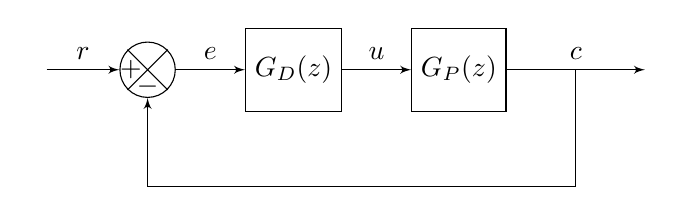
\begin{tikzpicture}
                    \sbEntree{in}
                    \sbComp{comp}{in}
                    \sbRelier[$r$]{in}{comp}
                    
                    \sbBloc[2.5]{control}{$G_{D}(z)$}{comp}
                    \sbRelier[$e$]{comp}{control}
        
                    \sbBloc[2.5]{system}{$G_P(z)$}{control}
                    \sbRelier[$u$]{control}{system}
                    
                    \sbSortie[5]{out}{system}
                    \sbRelier[$c$]{system}{out}
                    \sbRenvoi[3.5]{system-out}{comp}{}
                \end{tikzpicture}
                \legend{Fonte: do autor. }
            \end{figure}
            
            
            Para alcançar os requisito de projeto, precisamos definir a localização dos polos dominantes quando fecharmos a malha. 
            
            Para tal, pode-se utilizar uma relação analítica aproximada entre as figuras de mérito de um sistema de segunda ordem e os parâmetros de um sistema de segundo grau conhecidos como fator de amortecimento ($\zeta$) e frequência natural ($w_n$), conforme as \autoref{eq-zeta} e \autoref{eq-wn}. É importante salientar que são aproximações e que ao utilizarmos essas equações estamos admitindo uma margem de erro nos resultados do projeto. Para minimizar os efeitos de tais erros, aplica-se um fator de projeto, que aqui equivale a $2,5\%$ para o tempo de acomodação e $0,07\%$ para o sobressinal, ou seja, nos cálculos será utilizado um tempo de acomodação de $24,76\%$ e sobressinal de $8,045\%$, mas o sistema ainda será avaliado de acordo com os requisitos definidos na sessão anterior.
            
            Encontrou-se um $\zeta$ necessário de $0,6257$ e um $w_n$ de $209,41 [rad/s]$ para cumprir tais requisitos, ou seja, precisamos que os polos dominantes do sistema tenha uma boa equivalência com sistema de segunda ordem abaixo (\ref{eq-ftma_req}):
            
            \begin{equation}
                \label{eq-ftma_req}
                H_{req} = \frac{43850}{s^2 +262,1\,s + 43850}
            \end{equation}
        
            \subsubsection{Taxa de Amostragem}
            
                Como projetaremos um controlador digital, precisamos definir a taxa de amostragem que será empregada. Como uma regra geral, pode-se considerar que o controlador precisa de um bom número de amostras durante o tempo de subida do sinal desejado para realizar as ações de controle. Neste viés, uma recomendação se dá por utilizar uma frequência de amostragem cerca de 8 a 10 vezes superior à frequência natural amortecida ($w_d$), que aqui é calculada como $163,34\,[rad/s]$, ou seja, uma frequência de $400Hz$ parece ser suficiente. 
                
                Neste ponto, o autor gostaria de deixar claro que houveram diversas iterações utilizando \textit{scripts} automatizados para projetar e testar o controle utilizando algumas taxas diferentes e chegou à conclusão que valores entre $500$ e $10kHz$ funcionavam bem, optando por ficar em \textbf{1kHz}. A percepção obtida é que, para esta planta, quanto maior a frequência, mais sensível à precisão do conversor analógico-digital o controlador se tornava, e quanto mais baixa a frequência, maior o valor máximo das ações de controle, chegando em saturações no sinal de \textit{PWM} aplicado.
                
                Utilizando tal frequência de amostragem aproximadamente 38 vezes maior que a frequência natural amortecida da planta, faz-se a amostragem da \autoref{eq-Gps} a partir de um segurador de ordem zero $ZOH$, resultando em \autoref{eq-Gpz}.
                
                \begin{equation}
                    \label{eq-Gps}
                    G_p(s) = \frac{7239000}{s^3 +722,4\,s^2 +78410\,s +7239000}
                \end{equation}
                
                \begin{equation}
                    \label{eq-Gpz}
                    G_p(z) = \frac{0,001013\,z^2 + 0,003402\,z + 0,0007061}{ z^3 -2,427\,z^2 +1,918\,z -0,4856}
                \end{equation}
                
                Para testar a equivalência, testou-se a partir de um \textit{script} a resposta dos sistemas no domínio contínuo ($S$) e discreto ($Z$), mostrados na \autoref{fig-step-gps-gpz}.
                
                \FloatBarrier
                \begin{figure}[htbp]
                	\centering
                	\caption{Resposta ao Degrau na Planta em Malha Aberta}
                	\includegraphics[width=\textwidth,height=240px,keepaspectratio]{imgs/ftma/step-gps-gpz.png}
                	\label{fig-step-gps-gpz}
                	\legend{Resposta ao degrau unitário da planta em $S$ e $Z$. Fonte: do autor. }
            	\end{figure}
                \FloatBarrier
        
            \subsubsection{Local do polo desejado}
        	
            	A partir da \autoref{eq-polo-z} calculamos a posição dos polos dominantes no plano Z como sendo aproximadamente $ P=0,865511 \pm 0,142649\,j $.
            	
            	\begin{equation}
            	    \label{eq-polo-z}
            	    P = e^{-Ts * \zeta * w_n} \, e^{\pm Ts\,w_n\,j}
            	\end{equation}
            	
            	Ou seja, para satisfazermos nossos requisitos de projeto precisamos que os polos dominantes do sistema em malha fechada estejam localizados conforme mostrado em \autoref{fig-zplane-Gpz}.
            	
            	\FloatBarrier
            	\begin{figure}[htbp]
                	\centering
                	\caption{Polos da planta em malha aberta em relação ao desejado de malha fechada}
                	\includegraphics[width=\textwidth,height=240px,keepaspectratio]{imgs/ftma/zplane-gpz.png}
                	\label{fig-zplane-Gpz}
                	\legend{Polos da planta em malha aberta em Preto, e polos dominantes de malha fechada desejados, em Azul. Fonte: do autor. }
            	\end{figure}
            	\FloatBarrier
    	
        	\subsubsection{Estratégias para o Controlador}
        	
            	Para alcançar o requisito de erro nulo em regime permanente, um polo em $z=1$ é necessário. 
            	Podemos cancelar o par de polos dominantes do sistema com um par de zeros complexos em nosso controlador, e calcular um polo de malha aberta que resulte nos polos dominantes de malha fechada serem exatamente os polos dominantes desejados, ou seja, selecionamos um controlador avanço-atraso com um par complexo de zeros $\alpha$, um polo em $z=1$ para lidar com o erro e um polo adicional $\beta$, conforme mostra a \autoref{eq-controlador}.
            	
            	\begin{equation}
            	    \label{eq-controlador}
            	    G_D(z) = K\,\frac{(z+\alpha)(z+\alpha^*)}{(z-1)(z+\beta)}
            	\end{equation}
            	
            	Para que haja o cancelamento, temos $\alpha = 0,942996 +0,088960\,j$.
            	
            	Para que os polos desejados $ P=0,865511 \pm 0,142649\,j $ sejam o lugar das raízes, a soma dos ângulos de polos e zeros em relação à ele deve ser igual à $\pm 180^o$. Um \textit{script} (\autoref{ap-scripts}) foi programado para fazer tais cálculos. Um detalhe importante é que os polos e zeros já conhecidos do controlador foram adicionados neste somatório. Após a execução do algorítimo obteve-se:
            	
            	$$ \sum{\angle{p}} = -2,2542774744995544\,[rad] = -129,16058514023453^o$$
                $$ \sum{\angle{z}} = -1,6878597011287606\,[rad] = -96,7072372848905^o$$
                $$ \angle{\beta} = \sum{\angle{p}} -\sum{\angle{z}} \pm180 = 1,0043785534241032\,[rad] = 57,546652144655994^o $$
                $$\beta = real(P) -tan(\angle{\beta})\,imag(P) = 0,641193772122912$$
            	
            	O ganho $K$ pode ser determinado pela condição de módulo (\autoref{eq-modulo}), resultando em $K = 0,148765765461027$.
            
                \begin{equation}
                    \label{eq-modulo}
                    |G_D(z) G_P(z)|_{z = P} = 1
                \end{equation}
                
                Por fim resultamos com a função de transferência de um controlador (\autoref{eq-Gdz}) que levará os polos dominantes de malha fechada para exatamente a localização desejada P (conforme calculado em \autoref{eq-polo-z}).
                
                \begin{equation}
                    \label{eq-Gdz}
                    G_d(z) = \frac{4,149\,z^2 -7,825\,z +3,722}{z^2 -1,641\,z +0,6412}
                \end{equation}
                
                Computando a função de transferência de malha aberta e malha fechada conforme a topologia da planta (\autoref{fig-planta-blocos}), resultamos na \autoref{eq-ftma} e \autoref{eq-ftmf}.
                
                \begin{equation}
                    \label{eq-ftma}
                    FTMA(z) = 1\,FTMD(z) = G_D(z)\,G_P(z) = \frac{0,004202\,z^2 +0,01412\,z +0,002929}{z^3 -2,182\,z^2 +1,529\,z -0\,347}
                \end{equation}
                
                \begin{equation}
                    \label{eq-ftmf}
                    FTMF(z) = {FTMD(z)}{1 + FTMA(z)} = \frac{b(z)}{a(z)}
                \end{equation}
                
                Sendo:
                \begin{eqnarray*}
                    b(z) & = & 0,004202\,z^6 -0,001734\,z^5 -0,02783\,z^4\\
                    & &        +0,05027\,z^3 -0,02871\,z^2 +0,001449\,z +0,002358 \\
                    a(z) & = & z^7 -5,95\,z^6 + 15,11\,z^5 -21,21\,z^4 \\
                    & &        +17,73\,z^3 -8,818\,z^2 +2,407\,z -0,277
                \end{eqnarray*}
                
                Para testar o controlador, um degrau unitário foi aplicado no sistema em malha aberta e fechada e seus resultados podem ser vistos na \autoref{fig-step-ftma-ftmf}.
                
                \begin{figure}[htbp]
                	\centering
                	\caption{Repostas ao degrau do sistema}
                	\includegraphics[width=\textwidth,height=240px,keepaspectratio]{imgs/ftmf/step-ftma-ftmf.png}
                	\label{fig-step-ftma-ftmf}
                	\legend{Resposta ao degrau unitário do sistema em malha aberta e em malha fechada. Fonte: do autor. }
            	\end{figure}
                
                Medindo por meio de um \textit{script} (\autoref{ap-scripts}), temos a medição de um sobressinal de $7,7\%$ e um tempo de acomodação de $26\,[ms]$, aparentemente não atendendo o requisito de tempo de acomodação, que deveria ser menor ou igual a $25,4\,[ms]$, mesmo projetado com um certo fator.
                
                Neste ponto o autor reprojetou diversas vezes o controlador, combinando variações de requisitos de projeto juntamente com variações na frequência de amostragem (que não se mostrou influenciar significativamente), e por mais que o fator fosse aumentado, não havia uma diminuição significativa no tempo de acomodação, ou seja, o erro no cálculo do $\zeta$ utilizado no projeto não é linear e para este caso em específico o erro aumenta conforme diminuímos o requisito para o tempo de acomodação.
                
                Por fim optou-se por partir para testes práticos para avaliar o resultado com o controlador operando na planta real, que por sua vez pode ser ligeiramente diferente da planta modelada devido à precisão limitada das capturas do osciloscópio.
                
                Outra dificuldade interessante é que a planta foi levantada duas vezes durante o processo de reprojeto, pois nas quatro semanas decorridas desde que o projeto foi iniciado, os controladores que inicialmente desempenhavam bem passaram a ter sua performance degradada e o autor notou que a resposta ao degrau da planta havia modificado em termos cerca de 10\% em relação tempo de subida, valor e tempo de pico, sobressinal e também erro em regime permanente. 
                
                A mudança não prevista na planta atrasou o projeto significativamente até que o problema fosse percebido, pois praticamente todos os controladores que funcionavam pareciam ter a mesma performance, mesmo com projetos bastante diferentes, possivelmente havia um erro grande na estratégia de cancelamento dos polos, de modo que eles continuavam sendo os polos dominantes do sistema.
                
                A partir do momento em que o autor levantou pela segunda vez a planta, os resultados com os mesmos parâmetros se mostraram imediatamente melhores e só assim foi possível perceber a atuação significativa dos diferentes controladores reprojetados, na resposta do sistema.
            
                O autor desconhece o motivo real da anormalidade na planta, mas imagina que possa ter relação com o tema \textit{contaminação de substrato} - talvez estivesse com uma umidade maior perto da data da corrosão e montagem da placa, que foi quando a planta foi identificada pela primeira vez.
        
            \subsubsection{Equações Recursivas}
            
                Para que seja possível implementar o controlador em um microcontrolador, que irá atuar em cada amostra do valor de entrada e saída, é necessário levar a equação recursiva para a função de transferência do controlador, exatamente como um filtro de resposta infinita (\textit{IIR}).
                
                Realizando a transformada $Z$ inversa na equação para cada sinal \textbf{u}, \textbf{e} e \textbf{c} da planta (\autoref{fig-planta-blocos}), as equações recursivas foram obtidas, mostrados nas Equações \ref{eq-ck} à \ref{eq-ek}, sendo $G_{P_{a}}$ as raízes do denominador e $G_{P_{b}}$ do numerador da equação da planta $G_P$, e $G_{D_{a}}$ e $G_{D_{b}}$ o mesmo, mas para a equação do controlador.
                
                \begin{eqnarray}
                    \nonumber
                    c[k+3] & = & G_{P_{b}}[0]\,u[k+2] + G_{P_{b}}[1]\,u[k+1] + G_{P_{b}}[2]\,u[k] \\ \label{eq-ck}
                    & &        - G_{P_{a}}[1]\,c[k+2] - G_{P_{a}}[2]\,c[k+1] - G_{P_{a}}[3]\,c[k]
                \end{eqnarray}
                
                \begin{eqnarray}
                    \nonumber
                    u[k+3] & = & G_{D_{b}}[0]\,e[k+3] + G_{D_{b}}[1]\,e[k+2] + G_{D_{b}}[2]\,e[k+1] \\ \label{eq-uk} 
                    & &        - G_{D_{a}}[1]\,u[k+2] - G_{D_{a}}[2]\,u[k+1]
                \end{eqnarray}
                
                \begin{eqnarray}
                    \label{eq-ek}
                    e[k+3] = r[k+3] - c[k+3]
                \end{eqnarray}
                
                A partir destas equações um \textit{script} (\autoref{ap-scripts}) simulou o sistema a partir de uma entrada de um trem de degraus de $1$ a $1,5[V]$. O Resultado pode ser visto na \autoref{fig-step-recursive}, na qual também pode ser comparado com a resposta de malha aberta e malha fechada (utilizando as funções de transferência ao invés das equações recursivas).
                
                \FloatBarrier
                \begin{figure}[htbp]
                	\centering
                	\caption{Simulação de repostas ao degrau para o sistema digital}
                	\includegraphics[width=\textwidth,height=240px,keepaspectratio]{imgs/ftmf/step-recursive.png}
                	\label{fig-step-recursive}
                	\legend{Resposta ao degrau unitário do sistema em malha aberta e em malha fechada. Fonte: do autor. }
            	\end{figure}
                \FloatBarrier
                
                Aparentemente ocorre saturação na ação de controle \textbf{u}. O autor tentou uma diversidade de reprojetos variando a localização do polo desejado e a frequência de amostragem e por não haver variações significativas em seu valor, o autor optou por, novamente, avaliar os resultados na planta real.
            
            \subsubsection{Resultados}
            
                Um \textit{script}(\autoref{ap-scripts}) gerou as constantes utilizadas no \textit{firmware} implementado no \textit{DSP}. A resposta ao degrau para o sistema em malha fechada em comparação ao mesmo sistema em malha aberta pode ser visto na \autoref{fig-ftmf-step}.
                As formas de onda apresentam resultados similares aos esperados pela simulação da \autoref{fig-step-ftma-ftmf}.
                
                \begin{figure}[htbp]
                	\centering
                	\caption{Resposta ao Degrau na Planta em Malha Fechada e Aberta}
                	\includegraphics[width=\textwidth,height=240px,keepaspectratio]{imgs/ftmf/step_response.JPG}
                	\label{fig-ftmf-step}
                	\legend{Resposta ao degrau de $0,5\,[V]$ aplicado pela tensão média do \textit{PWM}. No Canal 1 (Amarelo) é a saída do sistema em malha fechada, o canal de referência A (Branco), representando a resposta ao degrau do sistema em malha aberta, e o canal 2 (azul), o \textit{trigger}. Fonte: do autor. }
            	\end{figure}
            	
            	O sinal da ação de controle \textbf{u}, que em simulação apresentou saturação, na prática, via ferramentas de \textit{debug} foi verificado que não passou de $1,6\,V$ para os degraus de $0,5\,[V]$ aplicados, chegando próximo dos $2,5\,[V]$ na inicialização do sistema, momento em que ocorre um degrau de $1\,[V]$.
            	
            	\FloatBarrier
                No \autoref{ap-ftmf} pode ser verificado a captura do osciloscópio para a obtenção de cada um dos parâmetros a seguir:
                $$V_{0}=1.0\,[V]$$
                $$V_{\infty}=1.51\,[V]$$
                $$t_{subida}=9,7\,[ms]$$
                $$t_{50\%}=8,2\,[ms]$$
                $$t_{s5\%}=25,6\,[ms]$$
                $$V_{pk}=1.54\,[V]$$
                $$t_{pk}=21,2\,[ms]$$
                $$M_{p}=5,88\%$$
                $$\zeta = 0,6697192 $$
                $$w_n = 199,5495 [rad/s]$$
                \FloatBarrier
                
                Utilizando a mesmo equação para descobrir a posição do polo desejado (\autoref{eq-polo-z} chega-se aos polos $P_{planta}= 0,865738 +0,129468\,j$, diferente do polo desejado $ P=0,865511 \pm 0,142649\,j $, resultando em um erro positivo de $0,78\%$ no tempo de acomodação obtido. A \autoref{tab-resultados} apresenta uma comparação de todos os dados obtidos durante o processo.
                
                \begin{table}[]
                    \label{tab-resultados}
                    \centering
                    \caption{Comparação dos resultados}
                    \begin{tabular}{r|c|c|c|c|c}
                            &               $Mp\%$&     $t_{s5\%}[ms]$&     $t_r\,[ms]$ &       $v_{\inf}$ &	$v_{\inf}$ \\ \hline
                        Bloco 1 nominal&    0 	  &     4,56 &              3,29 &              1,49 & 			0,999 \\
                        Bloco 1 antigo&     0 	  &     4,70 &              3,40 &              1,50 & 			 1,01 \\
                        Bloco 1 atualizado& 0 	  &     4,88 &              3,12 &              1,49 & 			0,996 \\
                        Bloco 2 nominal&    19,25 &     49,0 &              14,0 &              1,49 &	  	     1,00 \\
                        Bloco 2 antigo&     18,38 &     40,0 &              14,8 &              1,50 & 			 1,01 \\
                        Bloco 2 atualizado& 16,33 &     47,6 &              15,0 &              1,49 &			 1,00 \\
                        FTMA simulação  &   16,10 &     50,8 &              15,6 &              1,49 & 			0,999 \\
                        FTMA prático  &     16,32 &     49,2 &              15,2 &              1,49 & 			 1,01 \\
                        FTMF simulação  &   7,70 &      26,0 &              9,00 &              1,50 & 			 1,00 \\
                        FTMF prático  &     5,88 &      25,6 &              9,70 &              1,51 &			 1,00 \\
                        Requisitos	  &		8,05 &		25,4 &				N/A	&				N/A	&			N/A
                    \end{tabular}
                    \legend{Fonte: do autor.}
                \end{table}
                
                Neste ponto o autor vê algumas alternativas caso este erro seja intolerável: pode-se tentar um reprojeto com um fator de projeto maior para tentar obter um polo de malha fechada mais amortecido, pode-se variar o ganho do controlador K para compensar a localização do polo de malha fechada (que claramente não ficou exatamente no local desejado) ou pode-se levantar a planta com maior precisão para que a estratégia de cancelamento de polos seja mais efetiva.
                
                Em contra-partida, o tempo para realização do projeto restringe qualquer uma destas ações, de modo que o autor considera um resultado tolerável, dentro das diversidades encontradas no processo.

    \section{Conclusões}
    
        Neste trabalho surgiu uma série de desafios técnicos (muito mais que questões teóricas pertinentes à metodologia de alocação de polos) no qual o projetista teve que lidar, tomando certo tempo para investigação, compreensão e resolução que de modo algum apareceriam em exercícios de livros didáticos, e que dificilmente são comentados nos mesmos.
        
        Quanto aos resultados, vê-se que a localização do polo dominante de malha fechado projetado não ficou na posição nem durante as simulações, nem na prática, mostrando que um projeto seguindo esta metodologia deve ser feito com cautela, e possivelmente diversas iterações para buscando melhorias até cumprir os requisitos para a planta real, e se considerarmos uma planta com variações por conta da tolerância dos componentes, esta metodologia pode apresentar grandes dificuldades de ser implementada em um projeto industrial sem que seja necessário realizar ajustes para cada unidade de um suposto produto.
    
        O autor considera que o maior aprendizado neste processo foi compreender a influência dos erros de medição e dos desvios nas análises causados por aproximações em formulações e pensar sobre como lidar com eles. 
        
        Além disso, o autor cumpriu seu objetivo pessoal de realizar o trabalho inteiramente com software gratuitos, inclusive o sistema operacional (\textit{Linux}), utilizando principalmente o \textit{KiCAD} para o projeto da placa de circuito impresso, o pacote de controle \textit{python-control} da linguagem de programação \textit{Python}, o qual inclusive contribuiu adicionando a funcionalidade \textit{stepinfo}, equivalente à função de mesmo nome do \textit{MATLAB}, e por fim o \textit{LaTeX} para compilação deste relatório.
     
        Deste modo, o autor considera este projeto um processo de grande valor para a formação do estudante de engenharia eletrônica, que em exercício, atua com a interface entre a informação teórica e o que é concebível com a tecnologia e recursos disponíveis.
    
    
	% ---
	% Finaliza a parte no bookmark do PDF
	% para que se inicie o bookmark na raiz
	% e adiciona espaço de parte no Sumário
	% ---
	\phantompart
	
	% ---
	% Conclusão
	% ---
	%\section[Conclusões e recomendações]{Conclusões e recomendações}
	% ---
	

	% ----------------------------------------------------------
	% ELEMENTOS PÓS-TEXTUAIS
	% ----------------------------------------------------------
	\postextual
	
	% ----------------------------------------------------------
	% Referências bibliográficas
	% ----------------------------------------------------------
	%\pagebreak
	%\bibliography{modelo-referencias}
	
	% ----------------------------------------------------------
	% Glossário
	% ----------------------------------------------------------
	%
	% Consulte o manual da classe abntex2 para orientações sobre o glossário.
	%
	%\glossary
	
	% ----------------------------------------------------------
	% Apêndices
	% ----------------------------------------------------------
	
	% ---
	% Inicia os apêndices
	% ---
	\begin{apendicesenv}
	%	
	%	% Imprime uma página indicando o início dos apêndices
		\partapendices
	%	
% 		\chapter{questao1.m}
% 		\label{questao1.m}
% 		\lstinputlisting{questao1.m}
% 		\pagebreak

        \chapter{Códigos Fonte do Projeto}
            \label{ap-scripts}
            Por somar mais de 50 páginas, o autor opta por não incluir a listagem dos códigos fonte no relatório, deixando todos  eles abertos em licença GPL3, disponíveis em um repositório público no \textit{github} do autor.
            
            \url{http://github.com/joaoantoniocardoso/sct2_projeto1}
            
            Para facilitar o acesso, o código fonte deste documento \textit{LaTeX} podem ser acessados em:
            
            \url{http://github.com/joaoantoniocardoso/sct2_projeto1/tex}
            
            O código fonte do \textit{firmware} podem ser acessados em:
            
            \url{https://github.com/joaoantoniocardoso/sct2_projeto1/tree/master/f28335_ccs7/basic_F28335}
            
            O código fonte do \textit{hardware} podem ser acessados em:
            
            \url{https://github.com/joaoantoniocardoso/sct2_projeto1/tree/master/hardware/main}
            
            O código fonte para as simulações no \textit{LTSpice} podem ser acessados em:
            
            \url{https://github.com/joaoantoniocardoso/sct2_projeto1/tree/master/hardware/simulations}
            
            O código fonte dos \textit{scripts} em \textit{Python} e \textit{Jupyter Notebook} podem ser acessados em:
            
            \url{https://github.com/joaoantoniocardoso/sct2_projeto1/tree/master/projeto}
            
            Por fim, o repositório pode ser baixado como um arquivo compactado em extensão \textit{.zip} em:
            
            \url{https://github.com/joaoantoniocardoso/sct2_projeto1/archive/master.zip}
            
        \clearpage
	
    	\chapter{Capturas do Bloco de Primeira Ordem}
        	\label{ap-block1}
        	
        	\FloatBarrier
        	\begin{figure}[htbp]
            	\centering
            	\caption{Tempo de Subida}
            	\includegraphics[width=\textwidth,height=240px,keepaspectratio]{imgs/block1/rise_time.JPG}
            	\label{fig-block1-rise_time}
            	\legend{Resposta ao degrau de $0,5\,[V]$ aplicado pela tensão média do \textit{PWM}. No Canal 1 (Amarelo) é a saída do bloco de primeira ordem e o canal 2 (azul), o \textit{trigger}. Fonte: do autor. }
        	\end{figure}			
        
        	\begin{figure}[htbp]
            	\centering
            	\caption{Tempo de Acomodação}
            	\includegraphics[width=\textwidth,height=240px,keepaspectratio]{imgs/block1/settling_time.JPG}
            	\label{fig-block1-settling_time}
            	\legend{Resposta ao degrau de $0,5\,[V]$ aplicado pela tensão média do \textit{PWM}. No Canal 1 (Amarelo) é a saída do bloco de primeira ordem e o canal 2 (azul), o \textit{trigger}. Fonte: do autor. }
        	\end{figure}
        	
        	\clearpage
        	
        \chapter{Capturas do Bloco de Segunda Ordem}
        	\label{ap-block2}
        	
        	\FloatBarrier
        	\begin{figure}[htbp]
            	\centering
            	\caption{Tempo de Subida}
            	\includegraphics[width=\textwidth,height=240px,keepaspectratio]{imgs/block2/rise_time.JPG}
            	\label{fig-block2-rise_time}
            	\legend{Resposta ao degrau de $0,5\,[V]$ aplicado pela tensão média do \textit{PWM}. No Canal 1 (Amarelo) é a saída do bloco de segunda ordem e o canal 2 (azul), o \textit{trigger}. Fonte: do autor. }
        	\end{figure}			
        
        	\begin{figure}[htbp]
            	\centering
            	\caption{Tempo de Acomodação}
            	\includegraphics[width=\textwidth,height=240px,keepaspectratio]{imgs/block2/settling_time.JPG}
            	\label{fig-block2-settling_time}
            	\legend{Resposta ao degrau de $0,5\,[V]$ aplicado pela tensão média do \textit{PWM}. No Canal 1 (Amarelo) é a saída do bloco de segunda ordem e o canal 2 (azul), o \textit{trigger}. Fonte: do autor. }
        	\end{figure}
        
        	\begin{figure}[htbp]
            	\centering
            	\caption{Magnitude e Tempo de Pico}
            	\includegraphics[width=\textwidth,height=240px,keepaspectratio]{imgs/block2/overshoot.JPG}
            	\label{fig-block2-overshoot}
            	\legend{Resposta ao degrau de $0,5\,[V]$ aplicado pela tensão média do \textit{PWM}. No Canal 1 (Amarelo) é a saída do bloco de segunda ordem e o canal 2 (azul), o \textit{trigger}. Fonte: do autor. }
        	\end{figure}
        	\FloatBarrier
        	
        	\clearpage
    
        \chapter{Capturas da Planta em Malha Aberta}
        	\label{ap-ftma}
        	
        	\FloatBarrier
        	\begin{figure}[htbp]
            	\centering
            	\caption{Tempo de Subida}
            	\includegraphics[width=\textwidth,height=240px,keepaspectratio]{imgs/ftma/rise_time.JPG}
            	\label{fig-ftma-rise_time}
            	\legend{Resposta ao degrau de $0,5\,[V]$ aplicado pela tensão média do \textit{PWM}. No Canal 1 (Amarelo) é a saída da planta e o canal 2 (azul), o \textit{trigger}. Fonte: do autor. }
        	\end{figure}			
        
        	\begin{figure}[htbp]
            	\centering
            	\caption{Tempo de Acomodação}
            	\includegraphics[width=\textwidth,height=240px,keepaspectratio]{imgs/ftma/settling_time.JPG}
            	\label{fig-ftma-settling_time}
            	\legend{Resposta ao degrau de $0,5\,[V]$ aplicado pela tensão média do \textit{PWM}. No Canal 1 (Amarelo) é a saída da planta e o canal 2 (azul), o \textit{trigger}. Fonte: do autor. }
        	\end{figure}
        
        	\begin{figure}[htbp]
            	\centering
            	\caption{Magnitude e Tempo de Pico}
            	\includegraphics[width=\textwidth,height=240px,keepaspectratio]{imgs/ftma/overshoot.JPG}
            	\label{fig-ftma-overshoot}
            	\legend{Resposta ao degrau de $0,5\,[V]$ aplicado pela tensão média do \textit{PWM}. No Canal 1 (Amarelo) é a saída da planta e o canal 2 (azul), o \textit{trigger}. Fonte: do autor. }
        	\end{figure}
        	\FloatBarrier
        	
        	\clearpage
        	
        \chapter{Capturas da Planta em Malha Fechada}
        	\label{ap-ftmf}
        	
        	\FloatBarrier
        	\begin{figure}[htbp]
            	\centering
            	\caption{Tempo de Subida}
            	\includegraphics[width=\textwidth,height=240px,keepaspectratio]{imgs/ftmf/rise_time.JPG}
            	\label{fig-ftmf-rise_time}
            	\legend{Resposta ao degrau de $0,5\,[V]$ aplicado pela tensão média do \textit{PWM}. No Canal 1 (Amarelo) é a saída da planta e o canal 2 (azul), o \textit{trigger}. Fonte: do autor. }
        	\end{figure}			
        
        	\begin{figure}[htbp]
            	\centering
            	\caption{Tempo de Acomodação}
            	\includegraphics[width=\textwidth,height=240px,keepaspectratio]{imgs/ftmf/settling_time.JPG}
            	\label{fig-ftmf-settling_time}
            	\legend{Resposta ao degrau de $0,5\,[V]$ aplicado pela tensão média do \textit{PWM}. No Canal 1 (Amarelo) é a saída da planta e o canal 2 (azul), o \textit{trigger}. Fonte: do autor. }
        	\end{figure}
        
        	\begin{figure}[htbp]
            	\centering
            	\caption{Magnitude e Tempo de Pico}
            	\includegraphics[width=\textwidth,height=240px,keepaspectratio]{imgs/ftmf/overshoot.JPG}
            	\label{fig-ftmf-overshoot}
            	\legend{Resposta ao degrau de $0,5\,[V]$ aplicado pela tensão média do \textit{PWM}. No Canal 1 (Amarelo) é a saída da planta e o canal 2 (azul), o \textit{trigger}. Fonte: do autor. }
        	\end{figure}
        	\FloatBarrier
        	
        	\clearpage
	
	%	
	\end{apendicesenv}
	% ---
	
	% ----------------------------------------------------------
	% Anexos
	% ----------------------------------------------------------
	
	% ---
	% Inicia os anexos
	% ---
%	\begin{anexosenv}
%		
%		% Imprime uma página indicando o início dos anexos
%		\partanexos
%		
%	\end{anexosenv}
	
	%---------------------------------------------------------------------
	% INDICE REMISSIVO
	%---------------------------------------------------------------------
	
	\phantompart
	
	\printindex
		
\end{document}

